\uuid{3hfb}
\exo7id{7144}
\titre{exo7 7144}
\auteur{megy}
\organisation{exo7}
\datecreate{2017-04-05}
\isIndication{true}
\isCorrection{true}
\chapitre{Géométrie affine euclidienne}
\sousChapitre{Géométrie affine euclidienne du plan}

\contenu{
\texte{
Soit $\mathcal C$ un cercle et $P$ un point du plan. On considère une droite  $\mathcal D$ passant par $P$ et intersectant le cercle en au moins un point $E$. Soit $F$ le point diamétralement opposé à $E$. Montrer que $p_\mathcal C(P) = \overrightarrow{PE}\cdot \overrightarrow{PF}$.
\begin{center}
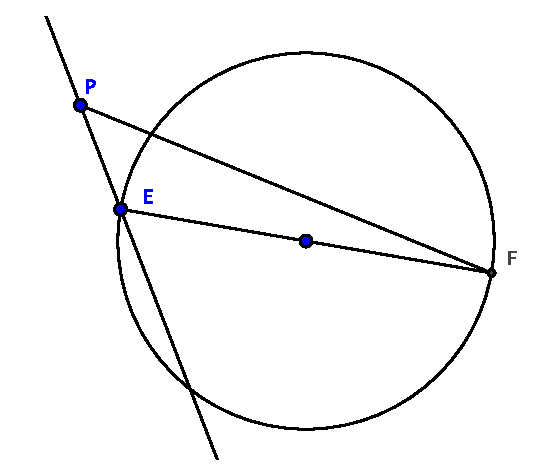
\includegraphics{../images/img007144-1}
\end{center}
}
\indication{Utiliser le second point d'intersection de la droite avec le cercle, s'il existe.}
\reponse{
Soit $G$ le projeté orthogonal de $F$ sur $\mathcal D$.

\begin{align*}
\overrightarrow{PE}\cdot \overrightarrow{PF}
&= \overrightarrow{PE}\cdot (\overrightarrow{PG}+\overrightarrow{GF})\\
&= \overrightarrow{PE}\cdot \overrightarrow{PG}
\end{align*}


Distinguons deux cas $ G=E$ et $G \neq E$. Dans le premier cas, cela signifie que le diamètre $(EF)$ est orthogonal à la droite $\mathcal D$, donc que celle-ci est tangente au cercle. Dans ce cas, $PE\cdot PG = PE^2$ est la puissance de $P$ par rapport au cercle.

Dans le deuxième cas, $EFG$ est rectangle en $G$, donc $G$ est sur le cercle de diamètre $[EF]$. On en déduit que $G$ est le second point d'intersection de $(PE)$ avec le cercle, et donc que $\overrightarrow{PE}\cdot \overrightarrow{PG}$ est là aussi la puissance de $P$ par rapport au cercle.


\begin{center}
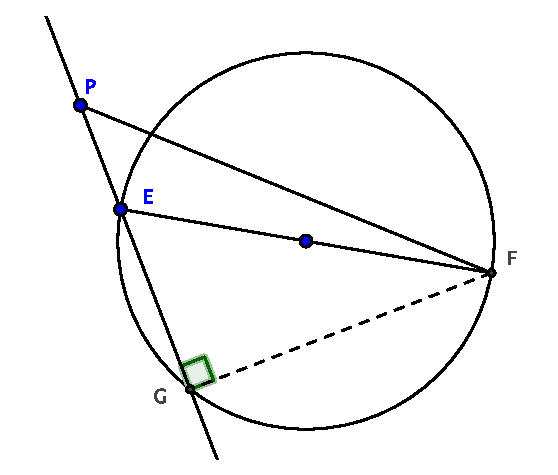
\includegraphics{../images/img007144-2}
\end{center}
}
}
